\documentclass[a4paper, 11pt]{article}
\usepackage[margin=1.1in]{geometry}

%use the english line for english reports
%usepackage[english]{babel}
\usepackage[portuguese]{babel}
\usepackage[utf8]{inputenc}
\usepackage{indentfirst}
\usepackage{graphicx}
\usepackage{verbatim}
\usepackage{fancyhdr}
\usepackage{listings}
\usepackage{color}

\definecolor{dkgreen}{rgb}{0,0.6,0}
\definecolor{gray}{rgb}{0.5,0.5,0.5}
\definecolor{orange}{rgb}{1,0.54,0}

\lstset{frame=tb,
  language=C,
  aboveskip=3mm,
  belowskip=3mm,
  showstringspaces=false,
  columns=flexible,
  basicstyle={\small\ttfamily},
  numbers=none,
  numberstyle=\tiny\color{gray},
  keywordstyle=\color{blue},
  commentstyle=\color{dkgreen},
  stringstyle=\color{orange},
  breaklines=true,
  breakatwhitespace=true,
  tabsize=3
}

\begin{document}

\setlength{\textwidth}{16cm}
\setlength{\textheight}{22cm}

\title{\Huge\textbf{2º Trabalho Laboratorial:}\linebreak\linebreak
\Huge\textbf{Rede de Computadores}\linebreak\linebreak\linebreak
\Large\textbf{Relatório}\linebreak\linebreak
\linebreak\linebreak

\includegraphics[scale=0.1]{images/feup-logo.png}\linebreak\linebreak
\linebreak
\Large{Mestrado Integrado em Engenharia Informática e Computação} \linebreak\linebreak
\Large{Redes de Computadores}\linebreak
}

\author{\textbf{Turma 1 Grupo 2:}\\
\linebreak\\
André Cruz - 201503776 \\
Bruno Piedade - 201505668 \\
Edgar Carneiro - 201503748 \\
\linebreak\linebreak \\
 \\ Faculdade de Engenharia da Universidade do Porto \\ Rua Roberto Frias, s\/n, 4200-465 Porto, Portugal \linebreak\linebreak
\linebreak\linebreak\vspace{1cm}}

\maketitle
\thispagestyle{empty}

%************************************************************************************************
%************************************************************************************************

\newpage

%Todas as figuras devem ser referidas no texto. %\ref{fig:codigoFigura}
%
%%Exemplo de código para inserção de figuras
%%\begin{figure}[h!]
%%\begin{center}
%%escolher entre uma das seguintes três linhas:
%%\includegraphics[height=20cm,width=15cm]{path relativo da imagem}
%%\includegraphics[scale=0.5]{path relativo da imagem}
%%\includegraphics{path relativo da imagem}
%%\caption{legenda da figura}
%%\label{fig:codigoFigura}
%%\end{center}
%%\end{figure}
%
%
%\textit{Para escrever em itálico}
%\textbf{Para escrever em negrito}
%Para escrever em letra normal
%``Para escrever texto entre aspas''
%
%Para fazer parágrafo, deixar uma linha em branco.
%
%Como fazer bullet points:
%\begin{itemize}
	%\item Item1
	%\item Item2
%\end{itemize}
%
%Como enumerar itens:
%\begin{enumerate}
	%\item Item 1
	%\item Item 2
%\end{enumerate}
%
%\begin{quote}``Isto é uma citação''\end{quote}

\tableofcontents

\newpage

%Sumário
\section{Sumário}
\normalsize 

Este trabalho foi realizado no âmbito da cadeira de Redes de Computadores, e visou o estudo de uma rede de computadores, da sua configuração e posterior ligação a uma aplicação desenvolvida pelo grupo. Para tal, além de seguir as recomendações e instruções fornecidas no guião, o grupo teve de fazer pesquisas acerca do funcionamento do protocolo FTP e respectiva ligação a um servidor. A aplicação desenvolvida permite ao utilizador fazer a transferência de um ficheiro fornecido por um \textit{URL}.

No final, é possível abordar as diversas conclusões obtidas estando estas relacionadas com os objetivos de cada uma das experiências, bem como com o desenvolvimento da aplicação.

%1. Introdução
\section{Introdução}

O projecto divide-se em duas grandes componentes: a configuração de uma rede de computadores; e o desenvolvimento de uma aplicação de download que permitisse o \textit{download} de um ficheiro através do protocolo \textit{FTP - File Transfer Protocol}.

O principal objectivo da configuração de rede é permitir a execução de uma aplicação, a partir de duas \textit{VLANs} dentro de um \textit{switch}. Numa das VLAN foi implementado o NAT, estando este activo, e na outra não, tendo esta última que conseguir ter ligação à \textit{Internet} para a aplicação de download funcionar correctamente.

Quanto aos objectivos da aplicação de download, era essencial o grupo entender o que é um cliente, um servidor e as suas características TCP/IP, bem como o funcionamente do protocolo FTP. Com estes objectivos concluídos, o grupo poderia avançar para o desenvolvimento da aplicação, implementando um cliente FTP e uma ligação TCP a partir de \textit{sockets}. Só então configuraríamos o servidor de DNS, para a conversão de um \textit{URL} para um IP, permitindo a sua localização num \textit{host} com domínio determinado.\\

%Assim, o trabalho tinha como objetivos:
%\begin{itemize}
%	\item compreender o conceito de `cliente - servidor' e entender as peculiaridades do protocolo de comunicação \textit{TCP/ IP};
%	\item compreender intrinsecamente o comportamento de: protocolos de aplicação em geral, de \textit{URL's - `Uniform Resource Locator' - } e do protocolo \textit{FTP};
%	\item localização e leitura de \textit{RFC's - `Request For Comments'};
%	\item a implementação de um cliente \textit{FTP} na linguagem de programação C;
%	\item uso de \textit{sockets} e de \textit{TCP - `Transmission Control Protocol' -} na linguagem de programação C;
%	\item compreender e fazer uso do serviço providenciado {DNS - `Domain Name System'}.\\
%\end{itemize}

O Relatório encontra-se dividido em diversas secções, nas quais se pode encontrar a seguinte informação:
\begin{itemize}
	\item \textbf{Arquitetura}, onde são descriminados os diferentes blocos funcionais e interfaces.
	\item \textbf{Estrutura do código}, apresentando as \textit{API}'s, principais estruturas de dados, principais funções e a sua relação com a arquitetura.
	\item \textbf{Casos de uso principais}, onde são identificados os principais casos de uso e as suas sequências de chamada de funções.
	\item \textbf{Aspetos Funcionais}, identificando os principais aspetos funcionais, bem como a descrição da estratégia de implementação.
	\item \textbf{Validação}, descrevendo os testes efetuados.
	\item \textbf{Experiências Laboratoriais}, onde é realizado um sumário de cada uma das experiências, bem como respondidas cada uma das perguntas relativas às experiências. De destacar que nas experiências quatro a seis, as respostas à pergunta já se encontram dentro do sumário da experiência para evitar grandes excertos de texto repetido.
	\item \textbf{Conclusões}, onde é feita uma tese da informação apresentada nas secções anteriores, bem como uma reflexão sobre os objetivos de aprendizagem alcançados.
\end{itemize}
%\pagebreak

% Parte 1
\section{Parte 1 - Aplicação de download}

%2.Arquitetura
\subsection{Arquitetura}

\large\textbf{Blocos Funcionais}\\
\normalsize
É possível distinguir a existência de dois blocos funcionais bem definidos: o bloco responsável pela validação e \textit{parsing} do \textit{URL} e o bloco responsável pela transferência de informação do servidor para o cliente. Os ficheiros \textit{URL.c} e \textit{URL.h} representam o primeiro bloco funcional referido, enquanto os ficheiros \textit{clientFTP.c} e \textit{clientFTP.h} representam o segundo bloco funcional referido. Cada um destes blocos será mais detalhadamente analisado em secções posteriores.
\newline

\large\textbf{Interface}\\
\normalsize
Na interface da linha de comandos é permitido ao utilizador correr o programa, apenas tendo de especificar como parâmetro qual o \textit{URL} do ficheiro a fazer \textit{download}.

%3.Estrutura do código & Aspetos Funcionais
\subsection{Estrutura do Código \& Aspetos Funcionais}

\large\textbf{\textit{URL Parsing}}\\
\normalsize

Tal como já foi referido na subsecção \textbf{Blocos Funcionais}, é nos ficheiros \textit{URL.c} e \textit{URL.h} que se faz a análise e interpretação do \textit{URL} que é passado como argumento na interface de comandos, aquando da execução do programa. Após a análise do \textit{URL} é preenchida uma estrutura de dados que guarda: o \textit{port} usado (será sempre o \textit{port} 21), o endereço \textit{IP - `Internet Protocol' - }, o diretório do ficheiro, o nome do \textit{host}, o nome do ficheiro, o nome utilizado para a autenticação do utilizador e a \textit{password} para a autenticação do utilizador.

\begin{lstlisting}[language=C]
typedef struct url_t {
  int port;
  char ip[URL_STR_LEN];          // host's ip
  char path[URL_STR_LEN];        // file path
  char hostname[URL_STR_LEN]; // hostname
  char filename[URL_STR_LEN]; // filename
  char username[URL_STR_LEN]; // username
  char password[URL_STR_LEN]; // password
} URL;
\end{lstlisting}

As  funções da \textit{\textbf{API}}, que também são as principais funções deste bloco funcional, são:

\begin{lstlisting}[language=C]
URL * constructURL();
int parseURL(URL* url, const char* str);
void setIp(URL * url);
void printURL(URL * url);
void destructURL(URL * url);
\end{lstlisting}

Como o nome indicada, a função \textit{constructURL} serve para criar a estrutura de dados.
A função \textit{parseURL} é a função responsável pelo \textit{parsing} e população de 5 dos 7 elementos da estrutura de dados, sendo que apenas o \textit{port} e o \textit{ip} não são populados. Assim, esta função tem como argumentos: um apontador para a estrutura \textit{URL} a ser populada, e a \textit{string} a ser analisada.
Para análise do \textit{URL} é utilizado um \textit{regex} por nós criado, sendo este:

\begin{lstlisting}[language=C]
#define URL_REGEX "^ftp://(([a-zA-Z][^:]*):([^@]+)@)?(([a-z0-9:]+[.]?)+)/(([^/]+[/])*)([^/]+)$"
\end{lstlisting}

É também feito uso de \textit{capture groups} de forma a capturar quais os elementos que se encontram a ser \textit{parsed} pelo \textit{regex}, para posteriormente serem guardados no lugar correto, dentro da estrutura de dados \textit{URL}. Assim à medida que o \textit{parser} encontra um elemento que corresponda a um \textit{capture group}, este é atualizado na estrutura de dados. Para tal efeito, usamos os seguintes importantes excertos de código: 

\begin{lstlisting}[frame=tlrb]
while (i++ < N_MATCHES) {
    int j = 0;
    int nomatch = regexec(r, p, N_MATCHES, m, 0);
    if (nomatch) {
        return i == 1 ? NO_MATCH : OK;
    }
    for (j = 0; j < N_MATCHES; j++) {
      int start = m[j].rm_so + (p - to_match);
      int finish = m[j].rm_eo + (p - to_match);

      setInUrl(url, j, to_match + start, finish - start);
    }
    p += m[0].rm_eo;
  }
\end{lstlisting}
\begin{lstlisting}[frame=tlrb]
static int setInUrl(URL * url, int idx, const char * src, int size) {
  switch (idx) {
    case 0: // whole capture
    case 1: // identity:password
    case 5: // host's country
    case 7: // path termination
      break;
    case 2: // username
      if (0 == size) {
        strcpy(url->username, "anonymous");
      } else {
        strncpy(url->username, src, size);
        url->username[size] = 0;
      }
      break;
    case 3: // password
      if (0 == size) {
        strcpy(url->password, "a");
      } else {
        strncpy(url->password, src, size);
        url->password[size] = 0;
      }
      break;
    case 4: // hostname
      strncpy(url->hostname, src, size);
      url->hostname[size] = 0;
      break;
    case 6: // path
      strncpy(url->path, src, size);
      url->path[size] = 0;
      break;
    case 8: // path
      strncpy(url->filename, src, size);
      url->filename[size] = 0;
      break;
    default:
      break;
  }
\end{lstlisting}

Continuando a análise das funções principais, a função \textit{setIp} permite a alteração do valor do campo \textit{ip} da estrutura de dados.
A função \textit{printURL} serve para imprimir os valores guardados na estrutura de dados para o ecrã.
Por fim, a função \textit{destructURL} serve para destruir a estrutura \textit{URL}.\\

\large\textbf{\textit{Download} do ficheiro}\\
\normalsize

Nos ficheiros \textit{clientFTP.c} e \textit{clientFTP.h} é feita a chamada às funções que executam a transferência do ficheiro desejado. Nestes, existe uma estrutura  que guarda os descritores dos ficheiros de controlo e de informação. O descritor do ficheiro de controlo é o local por onde é feita toda a comunicação com o servidor relativamente à configuração do \textit{download}, enquanto o descritor do ficheiro de informação é o local por onde é transmitido o ficheiro que o utilizador pretende fazer \textit{download}. Assim, faz sentido que toda a comunicação pelo canal de controlo seja feita antes da comunicação pelo canal de informação, de forma a garantir que todas as configurações se encontram corretas.

\begin{lstlisting}[language=C]
typedef struct ftp_t {
	int fdControl;
	int fdData;
} FTP;
\end{lstlisting}  

As  funções da \textit{\textbf{API}} deste bloco funcional são:

\begin{lstlisting}[language=C]
int downloadFtpUrl(const char * str);
\end{lstlisting}

Esta função recebe como argumento a \textit{string} correspondente ao \textit{URL} do ficheiro a ser transferido e caso o \textit{URL} seja válido, tenta executar essa transferência.\\

As principais funções deste bloco funcional são:

\begin{lstlisting}[language=C]
static int receiveCommand(int fd, char* responseCmd, char * expectedAnswer);
static int sendCommand(int fd, const char* msg, char* response, int readResponse, char * expectedAnswer);
static int connectSocket(const char* ip, int port);
static void retrieveFile(int fd);
static void sendUSER(int fd);
static void sendPASV(int fd);
static int download(int fd);
static void quitConnection();
\end{lstlisting}

As primeiras duas funções são as funções que merecem maior destaque pois é através destas que é feita toda a comunicação `cliente - servidor'.

 Assim, e como o nome o indica, a função \textbf{\textit{receiveCommand}}, permite receber uma resposta do servidor, sendo que esta será enviada através do descritor de ficheiro \textit{fd}.  No argumento \textit{expectedAnswer} é enviada a resposta que o cliente espera receber, sendo que se a resposta do servidor não corresponder à resposta que o cliente espera receber, é retornado erro. O argumento \textit{responseCmd}, se diferente de nulo, retorna a resposta do servidor. Internamente, é verificado se as respostas do servidor não são respostas de erro, pela análise do primeiro digito do código de retorno do servidor.

A função \textbf{\textit{sendCommand}} permite ao cliente enviar uma mensagem \textit{msg} ao servidor, através do descritor de ficheiro \textit{fd}, sendo que este devolve a resposta do servidor - \textit{response}. Verifica também se a resposta é semelhante à resposta esperada \textit{expectedAnswer}.

A função \textit{connectSocket} estabelece a comunicação entre o cliente e o servidor, pelo meio de \textit{sockets}, usando o \textit{ip} e o \textit{port} passados como argumento para definir essa ligação. Esta função retorna o descritor de ficheiro que ficará associado às comunicações.

A função \textit{retrieveFile} permite ao cliente pedir uma copia do ficheiro do qual este pretende fazer o \textit{download}. A comunicação é feita através do descritor de ficheiro de controlo \textit{fd}.

A função \textit{sendUSER} permite, através do descritor de ficheiro de controlo \textit{fd}, que o conjunto utilizador - \textit{password} seja autenticado pelo servidor.

A função \textit{sendPASV} permite que a comunicação \textit{FTP} com o servidor seja feita em modo passivo. A comunicação com o servidor é feita através do descritor de ficheiro de controlo \textit{fd}.

A função \textit{download} faz a transferência do ficheiro para o descritor de ficheiro de informação que lhe é passado como argumento.

A função \textit{quitConnection} termina todas as conexões existentes entre o cliente e o servidor.

%4. Casos de uso principais
\subsection{Casos de uso principais}

A funcionalidade de cada uma das funções mencionadas nesta secção foi previamente explicada na secção anterior, secção \textbf{Estrutura do Código}.

Existe unicamente um caso de uso: correr a aplicação de forma a fazer \textit{download} de um ficheiro, usando o protocolo de comunicação \textit{FTP}. Para correr a aplicação deve-se respeitar a chamada ao programa, que é feita através de:

\begin{lstlisting}[language=C]
printf( "\nUsage: %s ftp://[<user>:<password>@]<host>/<url-path>\n", argv[0]);
\end{lstlisting}

A sequência de chamada de funções é:
\begin{itemize}
	\item \textbf{downloadFtpUrl}, com argumento \textit{argv[1]};
	\begin{itemize}
		\item \textbf{constructURL};
		\item \textbf{parseURL}, com argumento \textit{argv[1]};
		\item \textbf{setIp};
		\item \textbf{connectSocket}, para o descritor de ficheiro de controlo;
		\item \textbf{sendUSER};
		\item \textbf{sendPASV};
		\item \textbf{connectSocket}, para o descritor de ficheiro de informação;
		\item \textbf{retrieveFile};
		\item \textbf{download};
		\item \textbf{destructURL};
		\item \textbf{quitConnection};
	\end{itemize}
\end{itemize}

%6. Validação
\subsection{Validação}

Para validação da aplicação desenvolvida e para garantir que funcionava de acordo com o protocolo especificado, foram realizadas constantemente testes durante o desenvolvimento do programa e também na sua demonstração. Foi testado o \textit{download} de ficheiros de diversos tamanhos, variando desde ficheiros de vários \textit {Kbytes} até ficheiros de \textit{Gbytes}, \textit{download} em modo anónimo e mode autenticado e a robustez do \textit{parser de URL} implementado.
%\pagebreak

%Parte 2. Experiências Laboratoriais
\section{Parte 2 - Configuração e análise da rede}

\subsection{Experiência 1 - Configurar uma rede IP}
Esta experiência teve como objetivo a configuração de IP’s em máquinas diferentes, de modo a que estas consigam comunicar entre si. Assim, após a configuração dos IP’s das portas eth0 de dois computadores e a adição das rotas necessárias à tabela de reencaminhamento, foi enviado um sinal \textit{ping} de um computador para o outro, para verificar que, de facto, as máquinas tinham uma ligação entre si.

Para a configuração dos computadores foi utilizado o comando \textbf{\textit{$<$ifconfig [ip]$>$}}, que atribui ao IP da interface o IP passado como argumento. Após esta configuração, executamos um ping de uma máquina para a outra com os IP’s definidos, operação essa que foi executada com sucesso. Foi também possível ver os pedidos ARP, com os pings definidos e a resposta da máquina correspondente com o seu endereço MAC.

\begin{figure}[h]
\centering
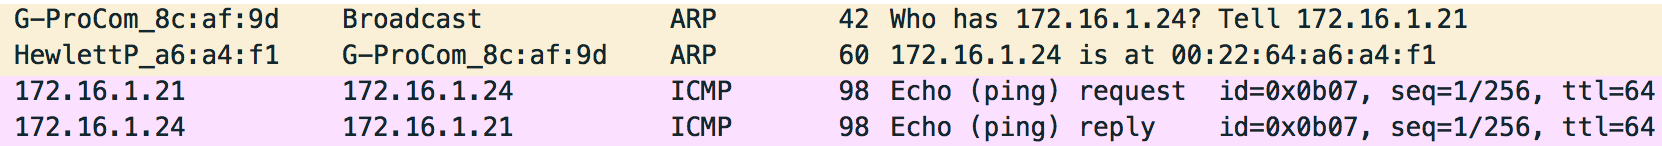
\includegraphics[scale=0.5]{images/Exp1_arp+ping.png}
\caption{Características dos pacotes enviados quando é iniciado um comando ping.}
\label{Momentanpol}
\end{figure}

\subsubsection{O que são os pacotes ARP e para que são usados?}
Os pacotes ARP (Address Resolution Protocol) são usados para mapear um endereço de rede (endereço IP) para um endereço físico (endereço MAC). Pode ver um exemplo das características dos pacotes ARP na figura 1.

\subsubsection{Quais são os endereços IP e MAC dos pacotes ARP?}
Os pacotes ARP têm como origem um IP / MAC já definido. No entanto, como destino têm ‘broadcast’ pois estes pacotes são emitidos para toda a rede local (LAN), tal como visível na figura 1.
Funcionamento: questionam à rede quem tem o IP X e esperam que o IP X responda dizendo:  o IP X está no MAC Y.

\subsubsection{Que pacotes são gerados aquando de um comando \textit{ping}?}
O comando ping gera pacotes de request (pedido de resposta) e reply (resposta) que seguem o protocolo ICMP (Internet Control Message Protocol) – ‘ICMP echo request packets’, tal como visível na figura 1.

\subsubsection{Quais são os endereços IP e MAC dos pacotes de \textit{ping}?}
Os pacotes ping ficam com o endereço IP e MAC de origem do computador de onde são enviados, e com o IP e MAC de destino dos computadores para os quais o ping é enviado (serve de exemplo a figura 1).

\subsubsection{Como é possível determinar se uma trama recebida é do tipo ARP, IP ou ICMP?}
Após o processo de \textit{demultiplexing} é obtido o cabeçalho da trama. Este \textit{header} tem uma correspondência única com cada protocolo, sendo, por exemplo, 0x0806 para as tramas do tipo ARP.

\subsubsection{Como é possível determinar o tamanho de uma trama recebida?}
O tamanho de uma trama só é descoberto após a descodificação total da mesma, num comportamento semelhante a strings com terminação em NULL em C. Assim, o último \textit{byte} de uma trama terá um valor especial que o sinaliza como tal.

\subsubsection{O que é e qual a importância da interface de \textit{loopback}?}
Uma interface de \textit{loopback} é uma interface de rede virtual que permite que um cliente e um servidor no mesmo host/computador comuniquem entre si usando a pilha de protocolos TCP/IP. Por convenção é usado o endereço IP 127.0.0.1 para esta interface.
Este mecanismo pode ser usado para testes de software ou de conectividade, permitindo verificar o funcionamento de parte da pilha TCP/IP num computador. Os pacotes enviados por esta interface nunca chegam à interface de rede física da máquina, o que permite testar software mesmo na ausência de tal interface de hardware.

% Exp2
\subsection{Experiência 2 - Implementar duas \textit{LAN}s virtuais no \textit{switch}}
O objetivo desta experiência era a criação de duas \textit{LAN}s virtuais no \textit{switch}: a primeira constituída pelas máquinas 1 e 4, e a segunda pela máquina 2. Com esta configuração, as máquinas 1 e 4 conseguem comunicar entre si, estando a máquina 2 isolada das restantes.

Foram efetuados comandos ping entre as máquina 1 e 4 e entre as máquinas 1 e 2, tendo este último falhado (como era de esperar), e o primeiro sido efetuado com sucesso, estando exposto na figura seguinte.

\begin{figure}[h]
\centering
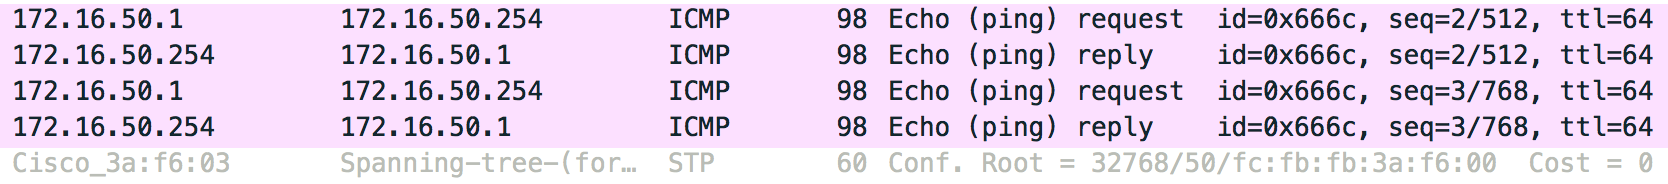
\includegraphics[scale=0.5]{images/ping1to4.png}
\caption{\textit{Logs} do comando ping com origem na máquina 1 e destino na máquina 4.}
\label{Momentanpol}
\end{figure}

\subsubsection{Configuração da vlan50}
Para a configuração de uma vlan, neste caso vlan50, tem primeiro de se criar a vlan. Para tal, tem de se criar ligações físicas entre os port do switch e os computadores que se prentede que façam parte da vlan . De seguida, no host que se encontra capaz de configurar o switch correm-se os seguintes comandos:
\begin{lstlisting}
configure terminal
vlan 50
end
\end{lstlisting}

Agora que a a vlan já se encontra criada, é necessário criar as ligações virtuais correspondentes às ligações físicas porta-computador. Para tal, no host configurador do switch, inserem-se os seguintes comandos:
\begin{lstlisting}
configure terminal
interface fastethernet 0/1
switchport mode access
switchport access vlan 50
end
\end{lstlisting}

Após a inserção desta configuração, passa a ser possível a comunicação entre os computadores configurados, através da vlan.

\subsubsection{Quantos \textit{broadcast domains} há?}
Existem dois \textit{broadcast domains}, um por cada \textit{vlan}/\textit{subnet}, como é possível averiguar através dos logs obtidos durante a execução do comando \textbf{ping -b \textless ip\textgreater} (broadcast) com origem na máquina 1 e na máquina 2.

% Exp3
\subsection{Experiência 3 - Configurar um router em \textit{Linux}}
Esta experiência tinha como objetivo a configuração da máquina 4 como um router entre as duas sub-redes criadas na experiência anterior.

Para este efeito, foi necessário ligar a interface \textit{eth1} - \textit{ethernet 1} - da máquina 4 e configurá-la com um IP dentro da mesma gama da máquina 2; adicionando, de seguida, esta interface à sub-rede da máquina 2.
\begin{figure}[h]
\centering
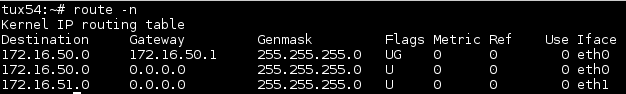
\includegraphics[scale=0.6]{images/Exp3_tux4_routing_table.png}
\caption{Configuração da \textit{routing table} da máquina 4.}
\label{Momentanpol}
\end{figure}

Após este passo, adicionou-se uma rota à máquina 1 utilizando o comando \textbf{\textit{$<$route add –net  172.16.y1.0/24 gw 172.16.y0.254$>$}}. O primeiro endereço identifica a gama de endereços para a qual se quer adicionar a rota; o segundo endereço identifica o IP para o qual se deve reencaminhar o pacote (neste caso o IP da máquina 4).
\begin{figure}[h]
\centering
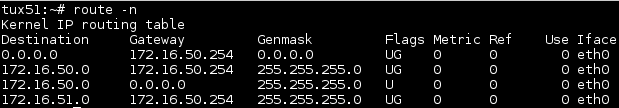
\includegraphics[scale=0.6]{images/Exp3_tux1_routing_table.png}
\caption{Configuração da \textit{routing table} da máquina 1.}
\label{Momentanpol}
\end{figure}

De seguida, repetiu-se o procedimento para a máquina 2, mas utilizando os seguintes endereços: \textbf{\textit{$<$route add –net 172.16.y0.0/24 gw 172.16.y1.253$>$}} (sendo o IP 172.16.y1.253 o endereço da máquina 4 nesta sub-rede).
\begin{figure}[h]
\centering
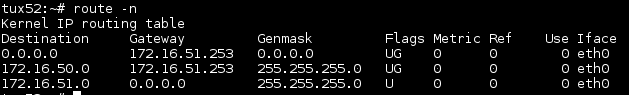
\includegraphics[scale=0.6]{images/Exp3_tux2_routing_table.png}
\caption{Configuração da \textit{routing table} da máquina 2.}
\label{Momentanpol}
\end{figure}

Finalmente, foi possível enviar um comando \textit{ping} da máquina 1 para a máquina 2 com sucesso. O pedido para o IP da máquina 2 (172.16.y1.1), é reencaminhado para a máquina 4 (172.16.y0.254); como a máquina 4 está ligada à sub-rede de ambas as máquinas, consegue aceder à máquina 2 através da sua interface eth1, que está nessa sub-rede, e à máquina 1 através da sua interface eth0. Na resposta, o processo é idêntico, sendo o pacote reencaminhado da máquina 2 para a máquina 1, através da máquina 4.
\begin{figure}[h]
\centering
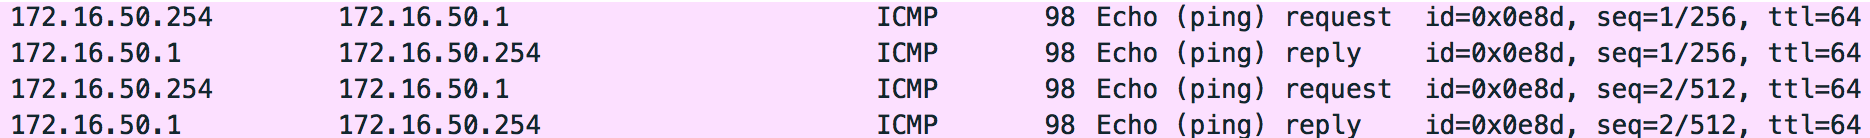
\includegraphics[scale=0.5]{images/Exp3_tux4eth0ping.png}
\caption{\textit{Logs} da interface \textit{eth0} da máquina 4.}
\label{Momentanpol}
\end{figure}
\begin{figure}[h]
\centering
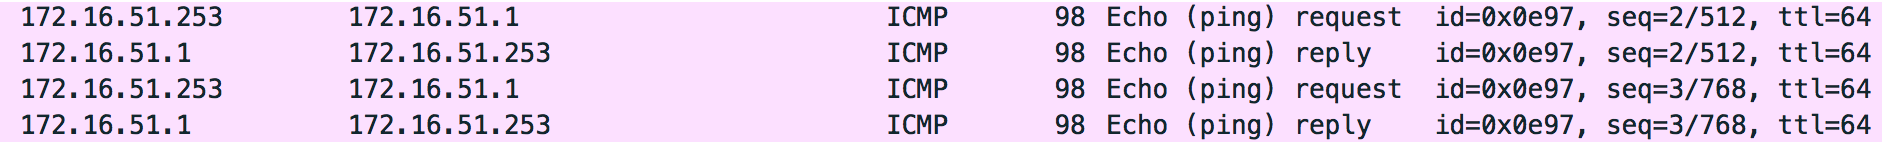
\includegraphics[scale=0.5]{images/Exp3_tux4eth1ping.png}
\caption{\textit{Logs} da interface \textit{eth1} da máquina 4.}
\label{Momentanpol}
\end{figure}

\subsubsection{Que rotas há nos \textit{tuxes}? E qual os seus significados?}
Em todos os tuxes existem redireccionamentos de rotas (ip forwarding). O redireccionamento de ip consiste no redirecionamento de pacotes através de um \textit{gateway} que tem acesso à origem e ao destino do respetivo pacote -neste caso o \textit{gateway} é o tux4. Assim, as rotas verificadsa nos tuxes são:

\begin{itemize}
\item tuxy1: redireccionamento do endereço IP do tuxy2 (.1) para o IP do router na respetiva vlan, tuxy4 (.254) – quanto tenta comunicar com o tuxy2 a mensagem é ao invés enviada para o tuxy4. Redireccionamento do endereço default IP para o endereço IP do router na respetiva vlan, tuxy4 (.254) – rota usada caso não seja encontrada mais nenhuma opção possível.
\item tuxy2: redireccionamento do endereço IP do tuxy1 (.1) para o IP do router na respetiva vlan, tuxy4 (.253) - quanto tenta comunicar com o tuxy1 a mensagem é ao invés enviada para o tuxy4. Redireccionamento do endereço default IP para o endereço IP do router na respetiva vlan, tuxy4 (.253) – rota usada caso não seja encontrada mais nenhuma opção possível.
\end{itemize}

As referidas configurações de \textit{routing tables} são visíveis nas figuras 3 (para o tux4), 4 (para o tux1) e 5 (para o tux2).

\subsubsection{Que informação contém uma entrada na \textit{forwarding table}?}
Uma linha da \textit{forwarding table} contém informação relativamente a: destino da mensagem (para onde foi pedido que a mensagem fosse enviada); gateway, para onde a mensagem será verdadeiramente enviada/redirecionada; genmask, a mascara de rede para a rede de destino; iface, a interface para a qual o pacote será enviado; e outras informações não tão relevantes como: ref, metric e use.

\subsubsection{Que mensagens ARP, e endereços MAC associados, são observados?}
Na tentativa do tuxy1 dar ping ao tuxy2, é possível verificar a mensagem ARP em que o tuxy4 pede o endereço MAC relativo ao IP do tuxy2.
O tuxy1 envia a informação para o tuxy2, sendo esta redirecionada para o tuxy4 através da tabela de rooting. 
Visto o tuxy4 não possuir na sua tabela ARP o endereço MAC do tuxy2 este necessita de transmitir (broadcast) um pacote ARP para descobrir esse endereço MAC.
\begin{figure}[h]
\centering
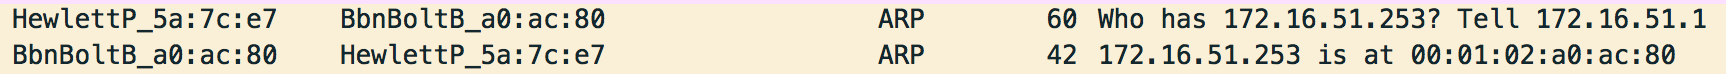
\includegraphics[scale=0.5]{images/Exp3_tux4eth1_ARPtux2.png}
\caption{Mensagens ARP capturadas na máquina 4, interface eth1.}
\label{Momentanpol}
\end{figure}

Na tentativa do tuxy2 dar ping ao tuxy1, irá acontecer um processo semelhante ao referido anteriormente, pelos mesmo motivos, sendo que neste caso o tuxy4 emitirá um pacote ARP para descobrir o endereço MAC do tuxy1.
\begin{figure}[h]
\centering
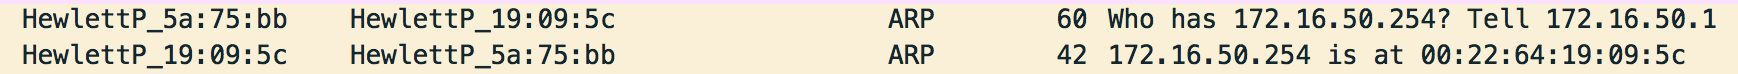
\includegraphics[scale=0.5]{images/Exp3_tux4eth0_ARPtux1.png}
\caption{Mensagens ARP capturadas na máquina 4, interface eth0.}
\label{Momentanpol}
\end{figure}

No início da comunicação, quer o tuxy1, quer o tuxy2 não sabem qual o endereço MAC do respetivo tuxy4 e, portanto, também emitem um pacote ARP para descobrir esse endereço (no caso do tuxy1 o .254 e no caso de tuxy2 o .253).
\begin{figure}[h]
\centering
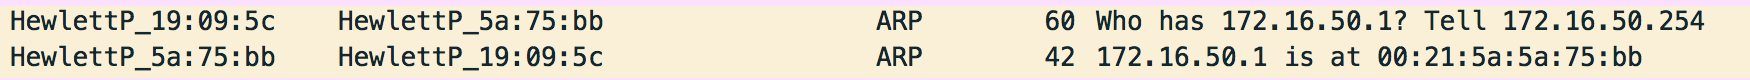
\includegraphics[scale=0.5]{images/Exp3_arp_messages.png}
\caption{Mensagens ARP capturadas na máquina 1.}
\label{Momentanpol}
\end{figure}

\subsubsection{Que pacotes ICMP são observados, e porquê?}
Na sequência da execução do comando ping no tux1, com o tux2 como destino, começa-se por verificar a existência de pacotes ICMP cujo endereço IP de origem é o tuxy1 e o endereço IP de destino é o tuxy2. No entanto, devido à possibilidade de \textit{forwarding}, esses pings passam a ser do tuxy1 para o tuxy4 \textit{.254}, e do tuxy1 para o tuxy4 \textit{.253} (ver figura 11).
\begin{figure}[h]
\centering
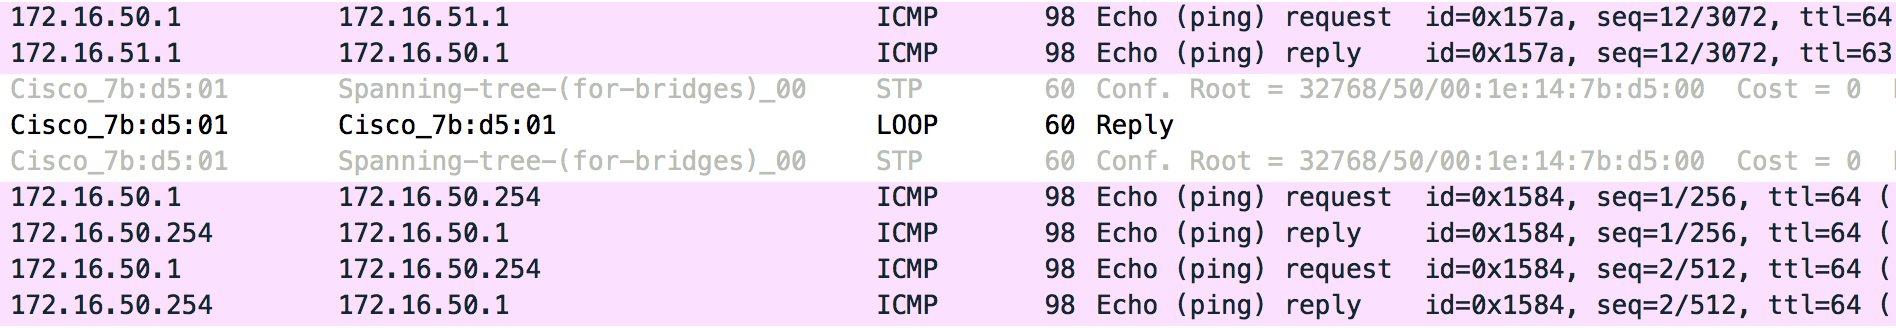
\includegraphics[scale=0.5]{images/Exp3_ICMP_packets_tux1.png}
\caption{Pacotes ICMP capturados no tux1.}
\label{Momentanpol}
\end{figure}

\subsubsection{Quais são os endereços IP e MAC associados aos pacotes ICMP?}
Os endereços MAC associados aos pacotes observados são os das respetivas máquinas de destino e origem (tux1 e tux4, respetivamente).
No entanto, devido ao \textit{forwarding} de pacotes pelo tux4, os pacotes podem ter endereço IP de destino correspondente ao do tux4 (terminado em 50.254 ou 51.253). Este facto é visualizado nas várias figuras de logs anteriores (6 a 11).

% Exp4
\subsection{Experiência 4 - Configurar um router comercial e implementar NAT}
O objetivo desta experiência era adicionar à sub-rede a ligação ao router e configura-lo com funcionalidades NAT de forma a estabelecer ligação à Internet. Para este objetivo foi necessário configurar duas \textit{interfaces} do router: interface \textit{gigabitEthernet 0/0} ligada à \textit{vlan1} e a \textit{interface gigabitEthernet 0/1} ligada à rede exterior da sala.

A partir da consola de configuração para ambas \textit{interfaces} foi definido o seu endereço IP e \textit{mask} através do comando \textbf{ip adress \textless ip\textgreater  \textless mask\textgreater} em que o IP era 172.16.51.254 para a \textit{interface 0/0} e 172.16.2.59 para a \textit{interface 0/1} com máscara de 24 bits. De seguida, introduziu-se o comando \textbf{no shutdown} para que as configurações não fossem perdidas caso o router fosse desligado e finalmente foi definido o ponto de entrada e saída de NAT através do comando \textbf{nat inside/outside} sendo aplicados respetivamente à \textit{interface 0/0} e \textit{interface 0/1}.

Após as \textit{interfaces} estarem configuradas, foi necessário executar os comandos \textbf{ip nat pool ovrld 172.16.2.59 172.16.2.59 prefix 24} e \textbf{ip nat inside source list 1 pool ovrld overload} para garantir a gama de endereços.

No seguimento, executou-se o comando \textbf{acesslist 1 permit ip  \textless max\textgreater} sobre ambas sub-redes - 172.16.50.0 e 172.16.51.0 – com o max definido com 0.0.0.255 para criar uma lista de acessos e permissões de pacotes.

Finalmente, definiu-se as rotas através do comando \textbf{ip route  \textless dest\textgreater  \textless mask\textgreater  \textless gw\textgreater} de forma a que os pacotes fossem redirecionados para o local correto. Foram adicionadas duas rotas: uma interna através do comando \textbf{ip route 0.0.0.0 0.0.0.0 172.16.1.254} para garantir que os pacotes eram enviados para a sub-rede 172.16.51.0 e uma rota externa através do comando \textbf{ip route 172.16.50.0 255.255.255.0 172.16.51.253} para garantir que os pacotes enviados para a sub-rede 172.16.50.0 eram redirecionados para o tuxy4 que estabelece ligação com esta sub-rede.

Adicionalmente foram utilizados os comandos   \textbf{route add} e   \textbf{ route del} para introduzir e remover, respetivamente, entradas nas listas de reencaminhamento e <traceroute [ip]> para analisar o percurso dos pacotes ao longo da rede.
\begin{figure}[h]
\centering
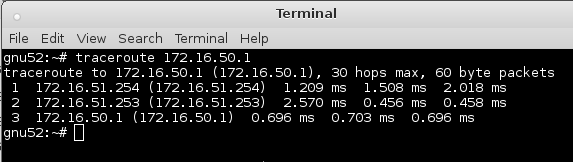
\includegraphics[scale=0.8]{images/Exp4_4traceroute.png}
\caption{Traceroute sem rota para sub-rede 172.16.50.0}
\label{Momentanpol}
\end{figure}
\begin{figure}[h]
\centering
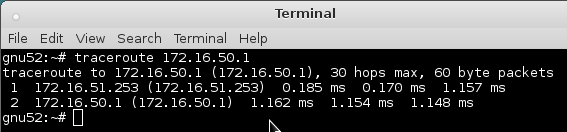
\includegraphics[scale=0.8]{images/Exp4_4traceroute2.png}
\caption{Traceroute com rota para sub-rede 172.16.50.0}
\label{Momentanpol}
\end{figure}


Através da análise dos resultados conclui-se que o router tem a capacidade de reencaminhar os pacotes para outras sub-redes quando no terminal não está definida a rota e que o a funcionalidade NAT é essencial à visibilidade da sub-rede para o exterior. 

% Exp5
\subsection{Experiência 5 - DNS}
Nesta experiência pretendia-se configurar o servidor de DNS para permitir ligação à Internet através da procura de nomes de domínios. Domain Name System (DNS) é responsável por associar e traduzir diversa informação associada aos nomes dos domínios em particular o seu IP.

Para associar o DNS à sub-rede foi necessário modificar o ficheiro \textit{/etc/resolv.conf} em todas as máquinas. Para tal, editou-se o seu conteúdo de acordo com o formato \textbf{search new-page-name  \textless nameserver\textgreater  \textless IP-page\textgreater}, sendo que \textit{new-page-name} representa o nome da página, e \textit{IP-page} o endereço IP da página.

O conteúdo do ficheiro passou a ser:

“search netlab.fe.up.pt 

 nameserver 172.16.2.1”

Para testar esta funcionalidade foi feito um ping ao domínio www.reddit.com.
\begin{figure}[h]
\centering
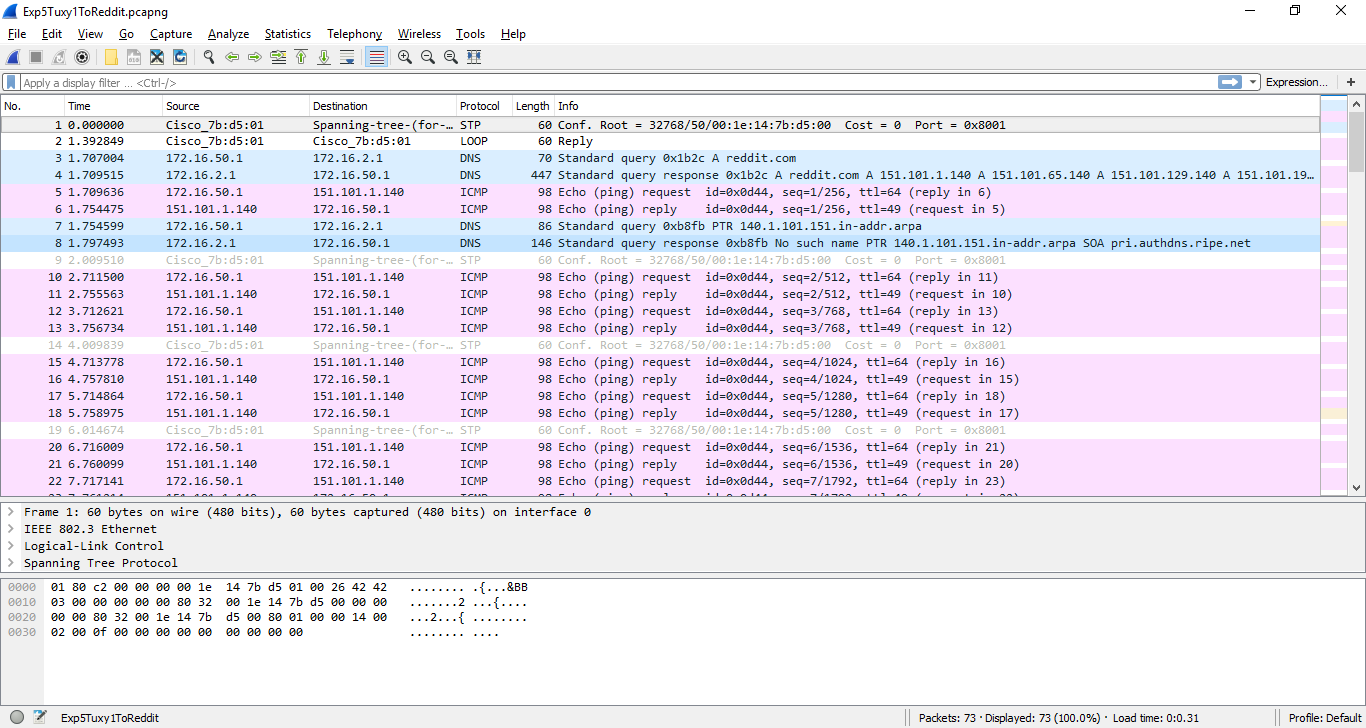
\includegraphics[scale=0.4]{images/Exp5_dns_packets.png}
\caption{Pacotes registados no ping a de reddit.com}
\label{Momentanpol}
\end{figure}

Através da análise dos resultados do \textit{Wireshark} podemos observar que no início da comunicação, antes do envio/receção de pacotes ICMP (enviados pelo comando \textbf{ping \textless ip\textgreater }), foram enviados pacotes DNS para identificar o endereço IP do destino (neste caso reddit.com). 

Foi pedido ao DNS que enviasse os atributos do domínio através do pacote 3. Como resposta o servidor enviou o pacote 4 que inclui entre outras informações o endereço IP do destino.

Posteriormente, foi também feito um pedido \textit{reverse} DNS (rDNS) nos pacotes 7 e 8 que processa o pedido contrário, ou seja, obter o nome domínio a partir do enderenço IP.

% Exp6
\subsection{Experiência 6 -Ligações  TCP}

Por fim, o objetivo desta experiência era desenvolver uma aplicação de download com base no protocolo FTP e analisar as características da comunicação tais como as ligações de controlo e dados e as suas fases, os dados transferidos através da ligação de controlo, o mecanismo ARQ e o mecanismo de controlo de congestão.

O mecanismo ARQ no TCP baseia-se numa variante de \textit{Go-Back-N} utilizando uma janela deslizante, em que são enviados \textbf{ACKs} com um único número de sequência para informar o emissor que os pacotes até esse número foram recebidos com sucesso. Em caso de erro ou perda de pacotes são enviados ACKs duplicados até que o emissor reenvie os pacotes perdidos um de cada vez (assunção otimista). É também utilizado timeout para quando uma resposta não é recebida. Este timeout é adaptativo, calculado dinamicamente de acordo com RTT (\textit{Round Trip Time}) medido ao longo da transmissão. Existe ainda a possibilidade de utilizar \textit{selective acknowledgements} (\textbf{SACKs}).
Para testar a aplicação foram feitas duas experiências. Em ambos os casos foi transferido um ficheiro com 758MB a partir do servidor ftp.up.pt.

Na primeira experiência a transferência foi feita a partir da maquina tuxy1.

Ao longo da execução da aplicação foram abertos dois canais de comunicação: um de controlo por onde são enviados vários comandos tais como \textbf{USER}, \textbf{PASV}, \textbf{RETR}, etc e um de dados por onde são recebidos os pacotes do ficheiro.

Podemos identificar 3 fases durante a comunicação: estabelecimento de conexão, transferência e terminação de conexão.
 A 1ª ocorre logo no inicio da transferência e é caracterizada por um handshake de 3 passos: envio de \textbf{SYN}, reposta de \textbf{[SYN, ACK]} e envio de \textbf{ACK}. Esta fase está visível na sequência dos pacotes 4-6 (Anexo I - figura 18).\\

A 2ª corresponde ao processo de transferência e é visível durante o envio e reposta de comandos FTP. Durante a transferência do ficheiro tornam-se evidentes várias características do TCP incluindo o mecanismo ARQ quando é pedido a retransmissão com pacotes duplicados (ex: pacote 62759  (Anexo I - figura 19)).\\

A 3ª ocorre no fim da transferência e é caracterizada por um handshake de 3 passos: envio de \textbf{ FIN}, resposta de \textbf{[FIN, ACK]}, envio de \textbf{ACK}. Esta fase está visível na sequência dos pacotes 875476-875478 \textbf{(ver Anexo I - figura 15 \& Anexo I - figura 20)}.

Através da analise do gráfico podemos concluir que o throughput inicialmente aumentou de forma linear até atingir um valor aproximado de 1300 pacotes/s e que se manteve em média por volta deste valor apenas com esporádicos decréscimos ao longo da transferência e por fim diminuiu novamente de forma linear.

O aspeto deste gráfico não está totalmente de acordo com nenhum dos algoritmos estudados, porém é possível detetar através do aumento linear rápido de throughput inicial que a janela de congestão estará a ser incrementada por um fator em cada RTT. 
É possível também analisar que deverá estar a ser utilizada a técnica de congestion avoidance já que após um decréscimo, são visíveis duas fases de incremento da janela de congestão: inicialmente mais rápida semelhante ao observado no início da transmissão e posteriormente mais lento, mas ainda linear.\\

Na segunda experiência foi feita a transferência a partir do tuxy1 e no decurso desta iniciou-se outra no tuxy2 \textbf{(ver Anexo I - figura 16 \& Anexo I - figura 17)}.

Através da análise dos gráficos podemos concluir que a transferência em simultâneo provocou um impacto no throughput da máquina 1, tendo em conta que se manteve em média por volta dos 1200 pacotes/s, ocorreram mais decréscimos e o tempo aumentou de 70s (registado na experiência anterior) para 74s.

Em relação à maquina 2, o resultado registado encontra-se mais próximo do teoricamente esperado. Porém, podemos analisar que o impacto da transferência da máquina 1 foi mínimo uma vez que a evolução do throughput manteve-se idêntica ao longo da transferência, mesmo após o tuxy1 ter terminado. 

%9. Conclusões
\section{Conclusões}

No final, foi possível concluir que a aplicação implementada era robusta e permitia um \textit{download} de ficheiros na sua integra e sem erros.

O grupo considera também que a realização e compreensão exaustiva das experiências traduziu-se posteriormente na facilidade de desenvolvimento da aplicação e na compreensão de todos os conceitos relativos ao projeto. Assim, é conclusão unânime que as experiências se revelaram uma grande fonte de conhecimento e parte mais complexa e trabalhosa do projeto.

O grupo considera ter dominado os objetivos implícitos no trabalho tais como: compreensão do conceito de `cliente - servidor', compreensão do protocolo de comunicação \textit{TCP / IP}, compreensão do protocolo de comunicação \textit{FTP}, compreensão do serviço \textit{DNS},compreensão do uso de \textit{sockets} e compreensão de como localizar e ler \textit{RFC}'s . O grupo considera que o desenvolvimento do protocolo consolidou os conhecimentos teóricos previamente adquiridos. 

\clearpage

%Anexo I
\section{Anexo I}
\begin{figure}[h]
\centering
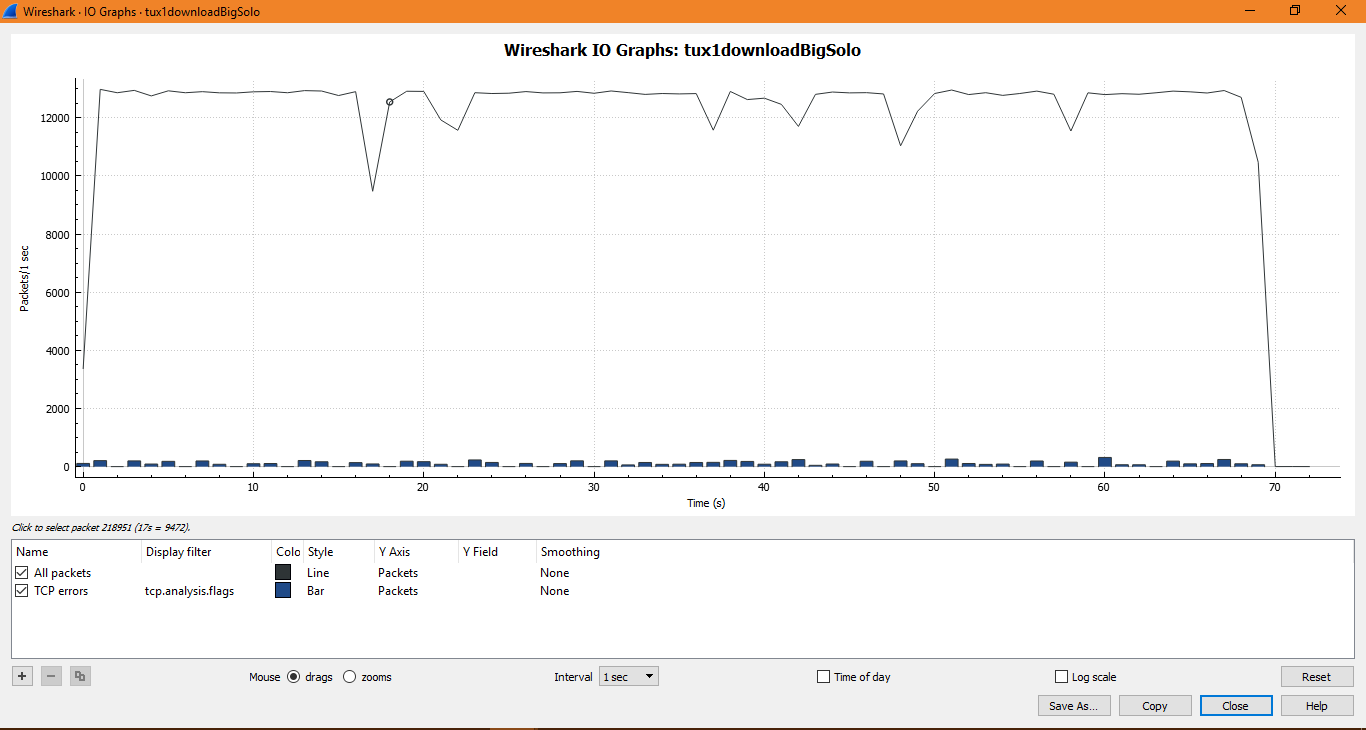
\includegraphics[scale=0.4]{images/tux1_solo_stats.PNG}
\caption{Variação de \textit{throughtput} de tuxy1}
\label{Momentanpol}
\end{figure}
\begin{figure}[h]
\centering
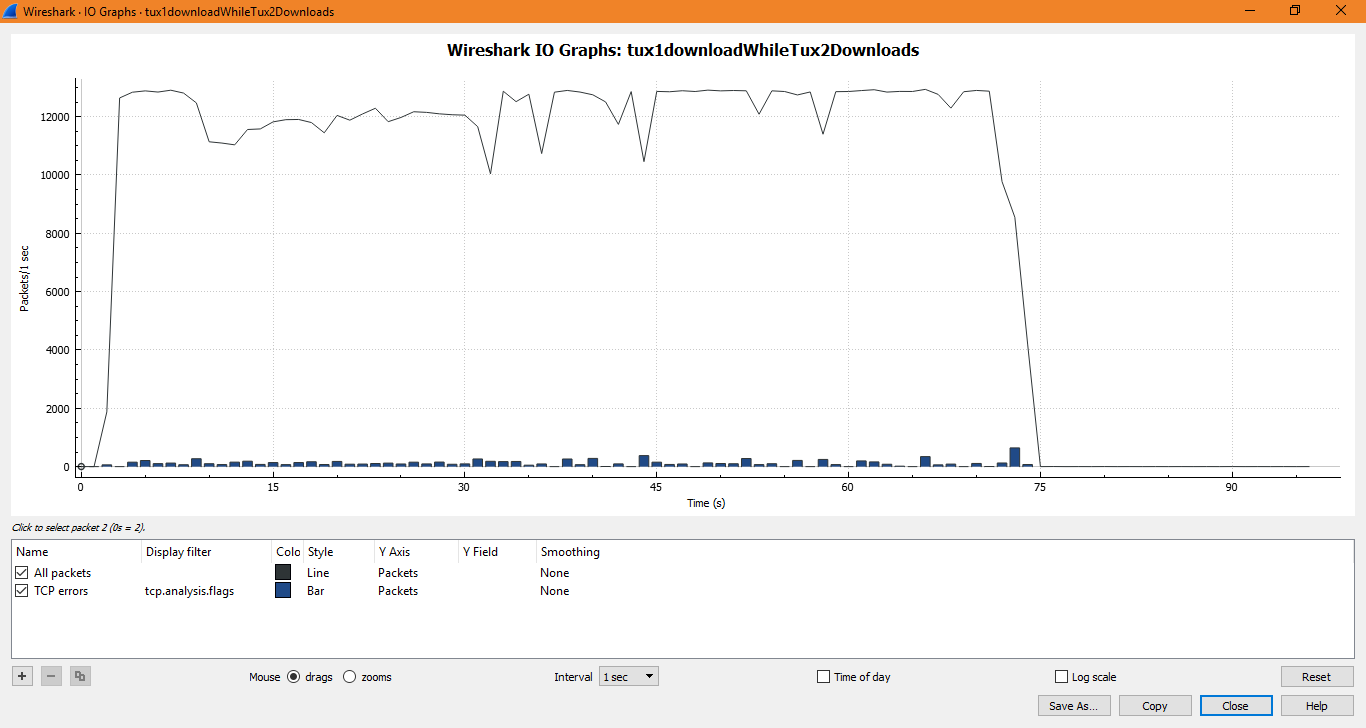
\includegraphics[scale=0.4]{images/tux1_while_tux2_stats.PNG}
\caption{Variação de \textit{throughtput} de tuxy1 durante transferência em simultâneo}
\label{Momentanpol}
\end{figure}
\begin{figure}[h]
\centering
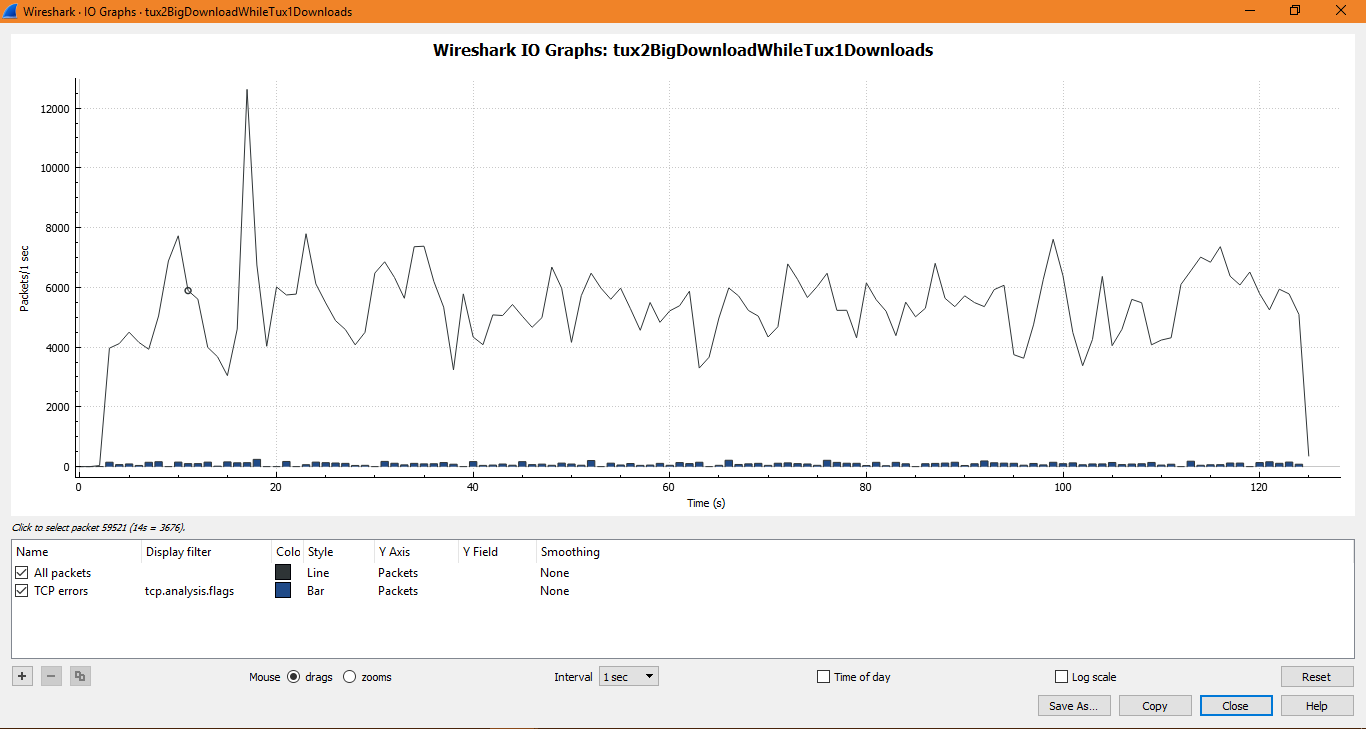
\includegraphics[scale=0.4]{images/tux2_while_tux1_stats.PNG}
\caption{Variação de \textit{throughtput} de tuxy2 durante transferência em simultâneo}
\label{Momentanpol}
\end{figure}
\begin{figure}[h]
\centering
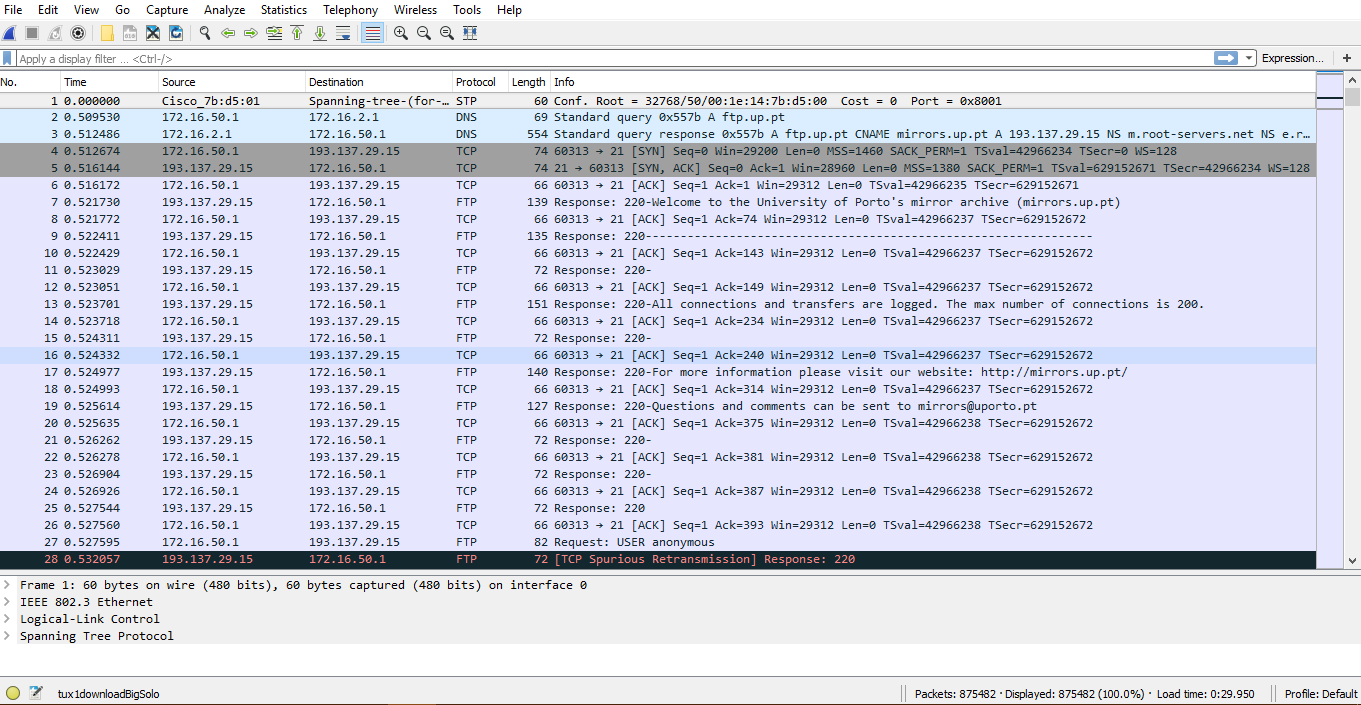
\includegraphics[scale=0.35]{images/tux1Solo_Inicio.png}
\caption{Início da transferência no tuxy1}
\label{Momentanpol}
\end{figure}
\begin{figure}[h]
\centering
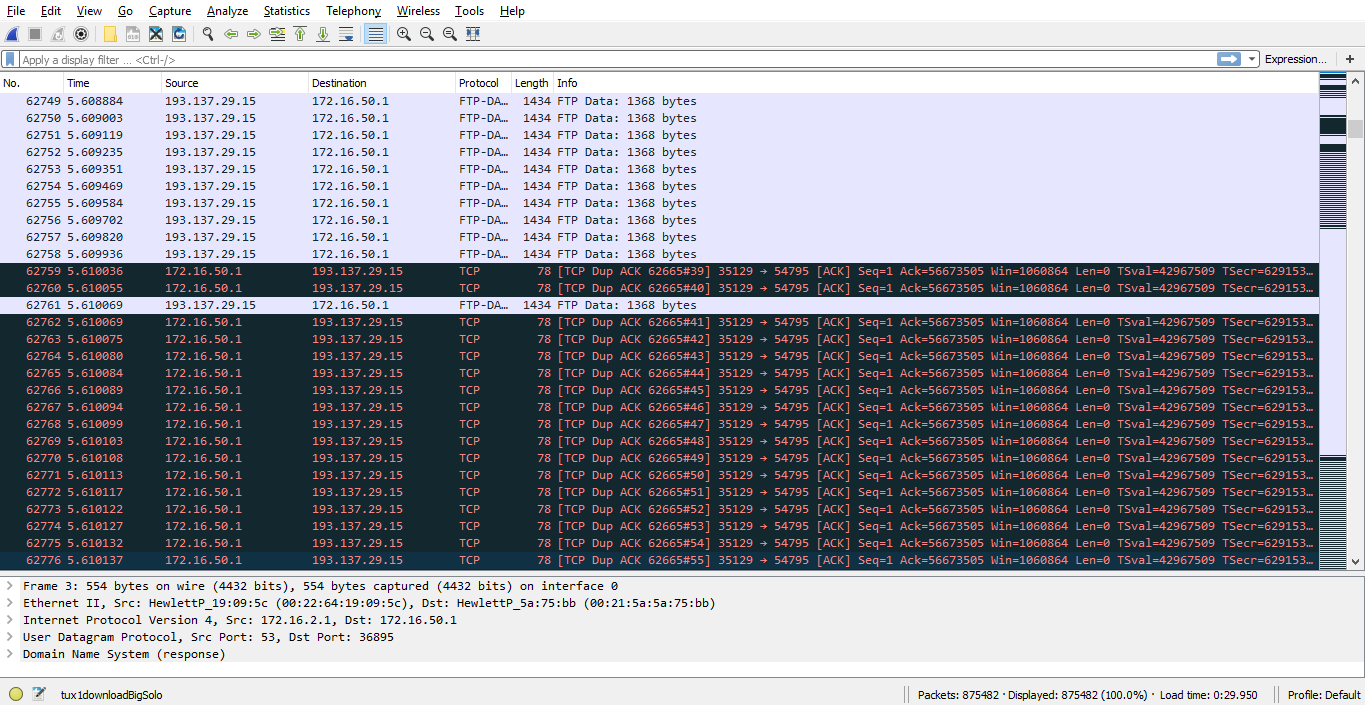
\includegraphics[scale=0.35]{images/tux1Solo_Inicio-Meio.png}
\caption{Transmissão de pacotes  \textit{dup ACK} durante transferência no tuxy1}
\label{Momentanpol}
\end{figure}
\begin{figure}[h]
\centering
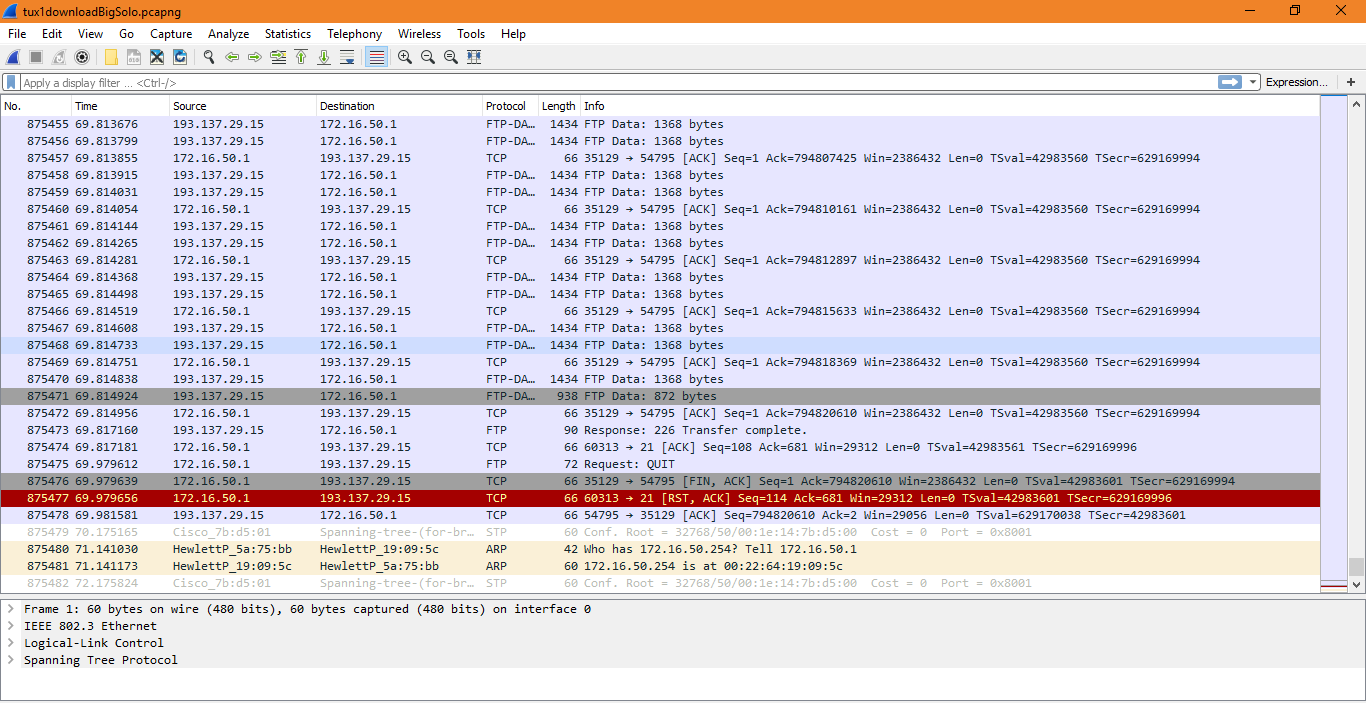
\includegraphics[scale=0.35]{images/tux1Solo_Fim-Mesmo.png}
\caption{Fim da transferência no tuxy1}
\label{Momentanpol}
\end{figure}


\clearpage

%Anexo II
\section{Anexo II}

\huge\textbf{main.c}
\begin{lstlisting}[language=C]
#include <stdio.h>
#include <sys/types.h>
#include <sys/socket.h>
#include <netinet/in.h>
#include <arpa/inet.h>
#include <stdlib.h>
#include <unistd.h>
#include <signal.h>
#include <netdb.h>
#include <string.h>
#include <regex.h>

#include "URL.h"
#include "utils.h"
#include "clientFTP.h"

#define BUFFER_SIZE 1024

void printUsage(char ** argv) {
	printf(
    "\nUsage: %s ftp://[<user>:<password>@]<host>/<url-path>\n",
		argv[0]);
}

int main(int argc, char** argv) {

  if (argc != 2) {
    printUsage(argv);
    exit(1);
  }

  downloadFtpUrl(argv[1]);

  return 0;
}
\end{lstlisting}
\newpage

\huge\textbf{clientFTP.h}
\begin{lstlisting}[language=C]
#ifndef __CLIENTFTP_H
#define __CLIENTFTP_H

#include <string.h>
#include <netdb.h>
#include <stdio.h>
#include <stdlib.h>
#include <regex.h>
#include <errno.h>
#include <unistd.h>
#include <sys/types.h>
#include <sys/socket.h>
#include <arpa/inet.h>
#include <netinet/in.h>
#include <string.h>
#include <sys/stat.h>
#include <fcntl.h>

#define DEBUG					0	

#define SERVER_READY      	"220"
#define TRANSFER_COMPLETE 	"226"
#define REQUIRED_PASSWORD	"331"
#define SUCCESS_LOGIN     	"230"
#define FINISHED	      	"150"
#define	PASSIVE_MODE	  	"227"
#define DIRECTORY_OK	  	"250"
#define SET_TYPE  			"200"

typedef struct ftp_t {
	int fdControl;
	int fdData;
} FTP;

int downloadFtpUrl(const char * str);

#endif /* __CLIENTFTP_H */
\end{lstlisting}
\newpage

\huge\textbf{clientFTP.c}
\begin{lstlisting}[language=C]
#include "clientFTP.h"
#include "URL.h"
#include "utils.h"

static FTP * ftp;
static URL * url;

static void quitConnection();

static void forceQuit(char * errorMSg){
	int errorStatus = logError(errorMSg);
	quitConnection();
	exit(errorStatus);
}

static void printResponse(char * responseCmd){
  	if(DEBUG)
    	printf("%s", responseCmd);
  	else {
    	int msgLength = strlen(responseCmd)-RESPONSE_CODE_OFFSET;
   		char * msgWithoutCode = (char *) malloc(msgLength);
    	memcpy(msgWithoutCode, responseCmd+RESPONSE_CODE_OFFSET, msgLength+1);
    	printf("%s", msgWithoutCode);
    	free(msgWithoutCode);
  	}
}

static int receiveCommand(int fd, char* responseCmd, char * expectedAnswer) {

	FILE* fp = fdopen(fd, "r");
	int allocated = 0;
	if(responseCmd == NULL) {
		responseCmd = (char*) malloc(sizeof(char) * MESSAGE_SIZE);
		allocated = 1;
	}
	do {
		memset(responseCmd, 0, MESSAGE_SIZE);
		responseCmd = fgets(responseCmd, MESSAGE_SIZE, fp);
		printResponse(responseCmd);
	}  while (!('1' <= responseCmd[0] && responseCmd[0] <= '5') || responseCmd[3] != ' ');

	char responseStatus = responseCmd[0];

	if(expectedAnswer != NULL && strncmp(expectedAnswer, responseCmd, strlen(expectedAnswer))){
		if(allocated)
			free(responseCmd);
		return ERROR;
	}

	if(allocated)
		free(responseCmd);

	return (responseStatus > '4');
}

static int sendCommand(int fd, const char* msg, char* response, int readResponse, char * expectedAnswer) {
	int nBytes = write(fd, msg, strlen(msg));
	if (readResponse) 
		return receiveCommand(fd, response, expectedAnswer);
	else return (nBytes == 0);
}

static int connectSocket(const char* ip, int port) {
	int	sockfd;
	struct	sockaddr_in server_addr;

	/*server address handling*/
	bzero((char*)&server_addr,sizeof(server_addr));
	server_addr.sin_family = AF_INET;
	server_addr.sin_addr.s_addr = inet_addr(ip);	/*32 bit Internet address network byte ordered*/
	server_addr.sin_port = htons(port);		/*server TCP port must be network byte ordered */

	/*open an TCP socket*/
	if ((sockfd = socket(AF_INET,SOCK_STREAM,0)) < 0) {
			perror("socket()");
			exit(0);
	}

	/*connect to the server*/
	if (connect(sockfd, (struct sockaddr *)&server_addr,sizeof(server_addr)) < 0){
			perror("connect()");
			return -1;
	}

	return sockfd;
}

static void retrieveFile(int fd) {

	char userCommand[MESSAGE_SIZE + 1];

	sendCommand(fd, "TYPE L 8\r\n", NULL, TRUE, SET_TYPE); //Setting type of file to be transferred -> local file
	sprintf(userCommand, "RETR %s%s\r\n", url->path, url->filename);
	if(sendCommand(fd, userCommand, NULL, TRUE, NULL) != OK)
		forceQuit("Failed to retrieve file. Terminating Program.");
}

static void sendUSER(int fd) {

	char userCommand[MESSAGE_SIZE + 1];
	char passCommand[MESSAGE_SIZE + 1];

	receiveCommand(fd, NULL, NULL);

	if (strcmp(url->username, "anonymous") == OK)
		printf("Logging in: anonymous mode.\n");
	else
		printf("Logging in: authentication mode");

	sprintf(userCommand, "USER %s\r\n", url->username);
	if(sendCommand(fd, userCommand, NULL, TRUE, REQUIRED_PASSWORD) != OK)
		forceQuit("Failed to log in, wrong username?\nTerminating Program.");


	sprintf(passCommand, "PASS %s\r\n", url->password);
	if(sendCommand(fd, passCommand, NULL, TRUE, SUCCESS_LOGIN) != OK)
		forceQuit("Failed to log in, wrong password?\nTerminating Program.");
}

static void sendPASV(int fd) {

	char response[MESSAGE_SIZE + 1];

	if(sendCommand(fd, "PASV\r\n", response, TRUE, PASSIVE_MODE) != OK)
		forceQuit("Failed to enter passive mode. Terminating program.");


	int remoteIP[6];
	char* data = strchr(response, '(');
	sscanf(data, "(%d, %d, %d, %d, %d, %d)", &remoteIP[0],&remoteIP[1],&remoteIP[2],&remoteIP[3],&remoteIP[4],&remoteIP[5]);
	sprintf(url->ip, "%d.%d.%d.%d", remoteIP[0],remoteIP[1],remoteIP[2],remoteIP[3]);
	url->port = remoteIP[4]*256+remoteIP[5];
}

static int download(int fd) {
	FILE* outfile;
	if( !(outfile = fopen(url->filename, "w")) )
		return logError("Unable to open file.");

	int dots = 0;
	printf("Downloading.");

	char buf[SOCKET_SIZE];
	int bytes;
	while ( (bytes = read(fd, buf, sizeof(buf))) != 0 ) {
		if (bytes < 0)
			return logError("Empty data socket, nothing to receive.\n");

		if ((bytes = fwrite(buf, bytes, 1, outfile)) < 0) {
			return logError("Unable to write data in file.\n");
		}

		printDownloadProgress(&dots);
	}

	fclose(outfile);

	printf("\rDownload finished with success.\n");

	return OK;
}

static void quitConnection() {

	printf("Closing connection with the server.\n");
	if(sendCommand(ftp->fdControl, "QUIT\r\n", NULL, FALSE, NULL) != OK) {
		close(ftp->fdData);
		close(ftp->fdControl);
		exit(logError("Failed to exit connection. Forcing exit.\n"));
	}

	close(ftp->fdData);
	close(ftp->fdControl);
}

int downloadFtpUrl(const char * str) {

	ftp = (FTP *) malloc(sizeof(FTP));

	url = constructURL();
	if (parseURL(url, str))
		exit(logError("Error parsing url. Please provide a valid url.\n"));
		
	setIp(url);

	printURL(url);

	if((ftp->fdControl = connectSocket(url->ip, url->port)) == 0)
		exit(logError("Failed to open control conection. Terminating Program.\n"));

	sendUSER(ftp->fdControl);
	sendPASV(ftp->fdControl);

	if((ftp->fdData = connectSocket(url->ip, url->port)) == 0)
		exit(logError("Failed to open data connection. Terminating Program.\n"));

	retrieveFile(ftp->fdControl);
	download(ftp->fdData);

	destructURL(url);
	quitConnection();
	free(ftp);

	printf("TERMINATING PROGRAM\n");

	return OK;
}
\end{lstlisting}
\newpage

\huge\textbf{URL.h}
\begin{lstlisting}[language=C]
#ifndef __URL_H
#define __URL_H

#define URL_STR_LEN 256

#include <string.h>
#include <netdb.h>
#include <stdio.h>
#include <stdlib.h>
#include <errno.h>
#include <sys/types.h>
#include <sys/socket.h>
#include <arpa/inet.h>
#include <netinet/in.h>

typedef struct url_t {
  int port;
  char ip[URL_STR_LEN];       // host's ip
  char path[URL_STR_LEN];     // file path
  char hostname[URL_STR_LEN]; // hostname
  char filename[URL_STR_LEN]; // filename
  char username[URL_STR_LEN]; // username
  char password[URL_STR_LEN]; // password
} URL;

/**
 * URL struct constructor
 */
URL * constructURL();

/**
 * Parses the url command to the given URL struct
 */
int parseURL(URL* url, const char* str);

/**
 * Sets the ip field from the URL struct
 */
void setIp(URL * url);

/**
 * Prints the contents of the URL struct to STDOUT
 */
void printURL(URL * url);

/**
 * URL struct destructor
 */
void destructURL(URL * url);

#endif /* __URL_H */
\end{lstlisting}
\newpage

\huge\textbf{URL.c}
\begin{lstlisting}[language=C]
#include <string.h>
#include <regex.h>
#include "URL.h"
#include "utils.h"

#define URL_REGEX "^ftp://(([a-zA-Z][^:]*):([^@]+)@)?(([a-z0-9:]+[.]?)+)/(([^/]+[/])*)([^/]+)$"

static int setInUrl(URL * url, int idx, const char * src, int size) {
  switch (idx) {
    case 0: // whole capture
    case 1: // identity:password
    case 5: // host's country
    case 7: // path termination
      break;
    case 2: // username
      if (0 == size) {
        strcpy(url->username, "anonymous");
      } else {
        strncpy(url->username, src, size);
        url->username[size] = 0;
      }
      break;
    case 3: // password
      if (0 == size) {
        strcpy(url->password, "a");
      } else {
        strncpy(url->password, src, size);
        url->password[size] = 0;
      }
      break;
    case 4: // hostname
      strncpy(url->hostname, src, size);
      url->hostname[size] = 0;
      break;
    case 6: // path
      strncpy(url->path, src, size);
      url->path[size] = 0;
      break;
    case 8: // path
      strncpy(url->filename, src, size);
      url->filename[size] = 0;
      break;
    default:
      break;
  }

  return OK;
}

/*
 * Match the string in "to_match" against the compiled regular
 * expression in "r", storing the values in the given URL*.
 */
static int match_url_regex(regex_t * r, const char * to_match, URL * url) {
  /* "p" is a pointer into the string which points to the end of the
     previous match. */
  const char * p = to_match;

  /* "N_MATCHES" is the maximum number of matches allowed. */
  const int N_MATCHES = 10;

  /* "m" contains the matches found. */
  regmatch_t m[N_MATCHES];

  int i = 0;
  while (i++ < N_MATCHES) {
    int j = 0;
    int nomatch = regexec(r, p, N_MATCHES, m, 0);
    if (nomatch) {
        return i == 1 ? NO_MATCH : OK;
    }
    for (j = 0; j < N_MATCHES; j++) {
      int start = m[j].rm_so + (p - to_match);
      int finish = m[j].rm_eo + (p - to_match);

      setInUrl(url, j, to_match + start, finish - start);
    }
    p += m[0].rm_eo;
  }

  return 0;
}

int parseURL(URL * url, const char* str) {
  regex_t r;
  const char * regex_text = URL_REGEX;
  int ret = 0;

  ret |= compile_regex(&r, regex_text);
  ret |= match_url_regex(&r, str, url);
  regfree(&r);

  return ret;
}

void printURL(URL * url) {
  printf("\nContents of URL struct:\n");
  printf("ip: %s\n", url->ip);
  printf("path: %s\n", url->path);
  printf("hostname: %s\n", url->hostname);
  printf("filename: %s\n", url->filename);
  printf("username: %s\n", url->username);
  printf("password: %s\n\n", url->password);
}

URL * constructURL() {
  URL * url = malloc(sizeof(URL));

  memset(url->ip, 0, URL_STR_LEN);
  memset(url->path, 0, URL_STR_LEN);
  memset(url->hostname, 0, URL_STR_LEN);
  memset(url->filename, 0, URL_STR_LEN);
  memset(url->username, 0, URL_STR_LEN);
  memset(url->password, 0, URL_STR_LEN);
  url->port = 21;

  return url;
}

void setIp(URL * url){
    memset(url->ip, 0, URL_STR_LEN);
    strcpy(url->ip, getIp(url->hostname));
}

void destructURL(URL * url) {
  free(url);
}
\end{lstlisting}
\newpage

\huge\textbf{utils.h}
\begin{lstlisting}[language=C]
#ifndef __UTILS_H
#define __UTILS_H

#include <sys/types.h>
#include <regex.h>

#define ERROR	    1
#define OK  	    0
#define NO_MATCH    2

#define TRUE		1
#define FALSE		0

#define SOCKET_SIZE				32768
#define MESSAGE_SIZE				1024
#define PATH_MAX					255
#define DOWNLOAD_PROGRESS_RESET	1000
#define RESPONSE_CODE_OFFSET		4

char * getIp(char * domain);

int compile_regex(regex_t * r, const char * regex_text);

void insertCharAt(char * dest, const char * src, char c, int size, int idx);

int logError(char * msg);

void printDownloadProgress(int * dots);

#endif /* __UTILS_H */
\end{lstlisting}
\newpage

\huge\textbf{utils.c}
\begin{lstlisting}[language=C]
#include <stdio.h>
#include <stdlib.h>
#include <string.h>
#include <errno.h>
#include <netdb.h>
#include <netinet/in.h>
#include <arpa/inet.h>
#include "utils.h"

#define MAX_ERROR_MSG 0x1000

/*
 * Compile the regular expression described by "regex_text" into "r".
 */
int compile_regex(regex_t * r, const char * regex_text) {
  int status = regcomp(r, regex_text, REG_EXTENDED|REG_NEWLINE);
  if (status != 0) {
  char error_message[MAX_ERROR_MSG];
  regerror (status, r, error_message, MAX_ERROR_MSG);
    printf ("Regex error compiling '%s': %s\n",
    regex_text, error_message);
    return 1;
  }
  return 0;
}

void insertCharAt(char * dest, const char * src, char c, int size, int idx) {
  if (idx >= size) return;
  strncpy(dest, src, size);
  memmove(dest + idx + 1, src + idx, size - idx);
  dest[idx] = c;
}

char * getIp(char * domain) {
  struct hostent *h;
  if ((h=gethostbyname(domain)) == NULL) {
      herror("gethostbyname");
      exit(1);
  }
  
  return inet_ntoa(*((struct in_addr *)h->h_addr));
}

int logError(char * errorMsg) {
  fprintf(stderr, "Error: %s\n", errorMsg);
  return ERROR;
}

void printDownloadProgress(int * dots) {
  (*dots)++;

  if(*dots == 3*DOWNLOAD_PROGRESS_RESET){
    *dots = 0;
    printf("\r                  ");
    printf("\rDownloading.");
  }
  else if(((*dots)%DOWNLOAD_PROGRESS_RESET) == 0)
    printf(".");

  fflush(stdout);
}
\end{lstlisting}
\newpage

\end{document}
